\chapter{总结与展望}
\section{工作归纳}

\begin{figure}[!ht]
    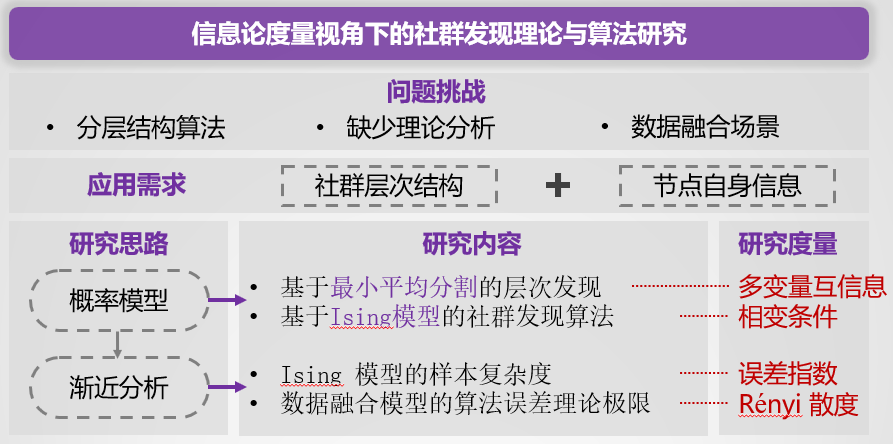
\includegraphics[width=0.9\linewidth]{screenshot-20230130-193759.png}
\end{figure}

\section{分析技术评注}
本文综合运用了多种信息论
度量研究社团发现问题。
它们均是针对
概率分布的距离度量,可总结为下表
\begin{table}[!ht]
    \centering
  \begin{tabular}{ccp{5cm}}
    \hline
     度量名称    &   参数个数 &   本文所处理的分布 \\
    \hline
     多变量互信息 &    $\geq 2$ &    弱独立的随机变量  \\
     速率函数     &    1 &     两个二项分布的差  \\
     雷尼散度     &    2 &    泊松分布和字母集有限的离散型随机变量(额外信息) \\
    \hline
  \end{tabular}
  \caption{各种信息论度量的对象}\label{tab:info_metric}
\end{table}
  
\section{研究展望}
本文的研究可在多方面进行拓展。

在算法设计层面,由于实际处理的图的规模可能比较大,
我们可以考虑HPSP,梅特罗波利斯算法的并行化。
而在研究玻茨模型的相变性质层面,我们可以从分布
\eqref{eq:isingma}独立采集多个
样本,通过系综学习(如多数同意规则)的方式进行社团发现,
然后研究相变点$\beta$和样本数的关系。

此外,本文研究的是带有额外信息的两社团随机块模型,
该研究思路有望拓展到其他随机图模型或多社团随机块模型上,并
通过似然函数构建类似\eqref{eq:matrix_mle}式
的优化目标,从而指导
一般性的有额外信息的图模型的
算法设计。然后我们可以将该方法与通过其他准则\cite{chunaev2020community}构建的算法进行
比较探索其适用场景。

另一方面,随着深度学习技术的兴起,社团发现任务亦可由
神经网络模型藉以完成,尤其是在有额外信息的场景下 \cite{cao2018incorporating}。
仿照本文研究梅特罗波利斯算法、半正定方法的思路,
未来可研究神经网络模型在随机块模型上的恢复误差,即可解释性问题。